\documentclass[journal]{IEEEtran}

\usepackage[pdfpagemode={UseOutlines},bookmarks=true,bookmarksopen=true,
   bookmarksopenlevel=0,bookmarksnumbered=true,hypertexnames=false,
   colorlinks,linkcolor={blue},citecolor={blue},urlcolor={blue},
   pdfstartview={FitV},unicode,breaklinks=true]{hyperref}

% *** MATH PACKAGES ***
\usepackage{amsmath,amssymb}

% *** GRAPHICS RELATED PACKAGES ***
\ifCLASSINFOpdf
	\usepackage[pdftex]{graphicx}
	\graphicspath{{images/}}
	% \DeclareGraphicsExtensions{.pdf,.jpeg,.png}
\else
	\usepackage[dvips]{graphicx}
	\graphicspath{{images/}}
	% \DeclareGraphicsExtensions{.eps}
\fi

% *** SUBFIGURE PACKAGES ***
\ifCLASSOPTIONcompsoc
  \usepackage[caption=false,font=normalsize,labelfont=sf,textfont=sf]{subfig}
\else
  \usepackage[caption=false,font=footnotesize]{subfig}
\fi

\usepackage{listings,color}

\definecolor{dkgreen}{rgb}{0,0.6,0}
\definecolor{gray}{rgb}{0.5,0.5,0.5}
\definecolor{mauve}{rgb}{0.58,0,0.82}
\newcommand{\fsize}{\small}
%\newcommand{\fsize}{\tiny}
\newcommand{\tabsize}{4}

\lstset{frame=tb,
  language=C++,
%  aboveskip=0mm,
  belowskip=0mm,
  showstringspaces=false,
  columns=flexible,
  basicstyle={\fsize\ttfamily},
  numberstyle=\fsize\color{gray},
%  numbers=left,
  keywordstyle=\color{blue},
  commentstyle=\color{dkgreen},
  stringstyle=\color{mauve},
  breaklines=true,
  breakatwhitespace=true,
  tabsize=\tabsize
}

% correct bad hyphenation here
\hyphenation{op-tical net-works semi-conduc-tor}

\newcommand{\fref}[1]{\figurename~\ref{#1}}
\newcommand{\eref}[1]{(\ref{#1})}
\newcommand{\tref}[1]{\tablename~\ref{#1}}
\newcommand{\lref}[1]{LISTING~\ref{#1}}

\begin{document}

% paper title
\title{Advanced Digital System Design Report I}

% author names and IEEE memberships
\author{Group 6: Yubo~Zhi (yz4116), Jiayang~Sun (js11815)}

% The paper headers
\markboth{ADSD Design Coursework}%
{ADSD Design Coursework}

% make the title area
\maketitle

\begin{abstract}
This introduction lab aims to design a hardware accelerator module to calculate dot product with High Level Synthesis (HLS) language. The hardware implementation was optimised by various directives in HLS. The differences between software and hardware implementations were also evaluated in this excise.
\end{abstract}

\section{Introduction}

Dedicated hardware accelerators can perform a particular task faster then generalised software design. However, there are a few trade-offs associated with using hardware accelerators. In this exercise, an IP core was developed and optimised using Vivado HLS toolkit. It computes the dot product of 2 input vectors. The performance differences between hardware and software implementations were assessed and discussed.

%\IEEEPARstart{T}{he} whole design is divided into three main parts. The first part is to familiar with the design toolkit, and complete the examples from the tutorial. Furthermore,  Finally, writing a test program for camparing the total simulation time of hardware module and software module.

%\cite{cw}

\hfill \today

\section{Synthesis tutorial}
\subsection{Incompatibility between toolkit versions}

Most sections of the high level synthesis tutorial went through smoothly. However, the example code \texttt{zynq\_design\_test.c} given in the tutorial has some incompatibility issues with the \texttt{2016.4} toolkit version. The function prototypes of the IP core driver generated by the toolkit have minor differences with the example code.

For example, the header file included by the example code is \texttt{XHls\_macc.h} while the header file generated actually called \texttt{xhls\_macc.h}. Functions used by the example follows a pattern looks like \texttt{XHls\_macc\_SetA}, but the generated functions look like \texttt{XHls\_macc\_Set\_a}.

These were not vital issues, they can be easily solved by renaming the file name and function names in the source code.

\section{Dot product implementation}

\subsection{Initial design}

\lref{lst:dotp} shows the high level C code design of the dot product module.

\begin{lstlisting}[caption={High level synthesis design for dot product},captionpos=b,label=lst:dotp]
#include <stdint.h>
#include "dotproduct.h"

void dotProduct(data_t x[N], data_t y[N],
                data_t *output)
{
        data_t acc = 0;
        uint32_t i;
loop:   for (i = 0; i != N; i++)
                acc += x[i] * y[i];
        *output = acc;
}
\end{lstlisting}

\subsection{Test bench}

\lref{lst:dotp_tb} shows the test bench developed for validation of hardware implementation.

\begin{lstlisting}[caption={Test bench for the dot product module},captionpos=b,label=lst:dotp_tb]
#include <stdio.h>
#include <stdlib.h>
#include "dotproduct.h"

int main()
{
        FILE *fp = fopen("result.dat", "w");
        FILE *fpg = fopen("result.golden.dat", "w");
        data_t x[N], y[N];
        int i, j;
        srand(666);
        for (i = 0; i != 600; i++) {
                for (j = 0; j != N; j++) {
                        x[j] = rand();
                        y[j] = rand();
                }
                data_t out;
                // Execute the function
                dotProduct(x, y, &out);
                // Save the results.
                fprintf(fp, "%i %d\n", i, out);
                // Generate golden reference
                out = 0;
                for (j = 0; j != N; j++)
                        out += x[j] * y[j];
                // Save the results.
                fprintf(fpg, "%i %d\n", i, out);
        }
        fclose(fp);
        fclose(fpg);
        
        // Comparison between outputs and golden reference.
        ...
}
\end{lstlisting}

Random numbers was generated as the inputs. Then a reference software implementation calculates the desired outputs as golden reference, instead of having to prepare a golden reference file each time for different data sets before simulation.

The seed to the pseudo random sequence was initially produced from the current system time, by using a \texttt{time(NULL)} function. However, this fails the C/RTL co-simulation verification. This is because the toolkit executes the RTL simulation, caches the output, then checking with C simulation afterwards. The system time can be different between RTL and C simulation, results in different random seeds actually used by the simulations.

\subsection{AXI4-lite interfacing}

By adding directives, the input and output ports in the dot product module were connected to an AXI4-lite interface. The ARM processor can use this interface to communicate with the module.

A total of 4 \texttt{s\_axilite} directives were specified. 1 for function return interrupt and 3 for each of the input and output ports. \lref{lst:dotp_lite} shows the directives added to the source code.

\begin{lstlisting}[caption={AXI4-lite directives added to the dot product module},captionpos=b,label=lst:dotp_lite]
#pragma HLS INTERFACE s_axilite port=return
#pragma HLS INTERFACE s_axilite port=x
#pragma HLS INTERFACE s_axilite port=y
#pragma HLS INTERFACE s_axilite port=output
\end{lstlisting}

\subsection{Optimisation and resource utilisation}

The optimisation was done by specifying directives to the \texttt{for} loop in the module.

Two directives were possible for the loop, \texttt{PIPELINE} and \texttt{UNROLL}. \tref{tbl:dir} compares the influences of these directives.

\begin{table}[!ht]
	% increase table row spacing, adjust to taste
	\renewcommand{\arraystretch}{1.3}
	\caption{Comparison between loop optimisation directives}
	\label{tbl:dir}
	\centering
	% Some packages, such as MDW tools, offer better commands for making tables
	% than the plain LaTeX2e tabular which is used here.
	\begin{tabular}{llll}
		\hline
			& None	& Pipeline	& Unroll \\
		\hline
		Latency	& 71	& 17	& 7	\\
		Interval	& 72	& 18	& 8	\\
		Co-simulation (average)	& 203	& 151	& 138	\\
		\hline
		BRAM\_18K	& 0	& 0	& 0	\\
		DSP48E	& 4	& 4	& 40	\\
		FF	& 1478	& 1477	& 990	\\
		LUT	& 7340	& 7339	& 1580	\\
		\hline
	\end{tabular}
\end{table}

The latency values are based on a $100 MHz$ fabric clock. The latency of the module was improved significantly by applying either \texttt{PIPELINE} or \texttt{UNROLL} directives. Unrolling the loop gives the best performance figure which is only 7 clock cycles latency.

\begin{figure*}[!t]
	\centering
	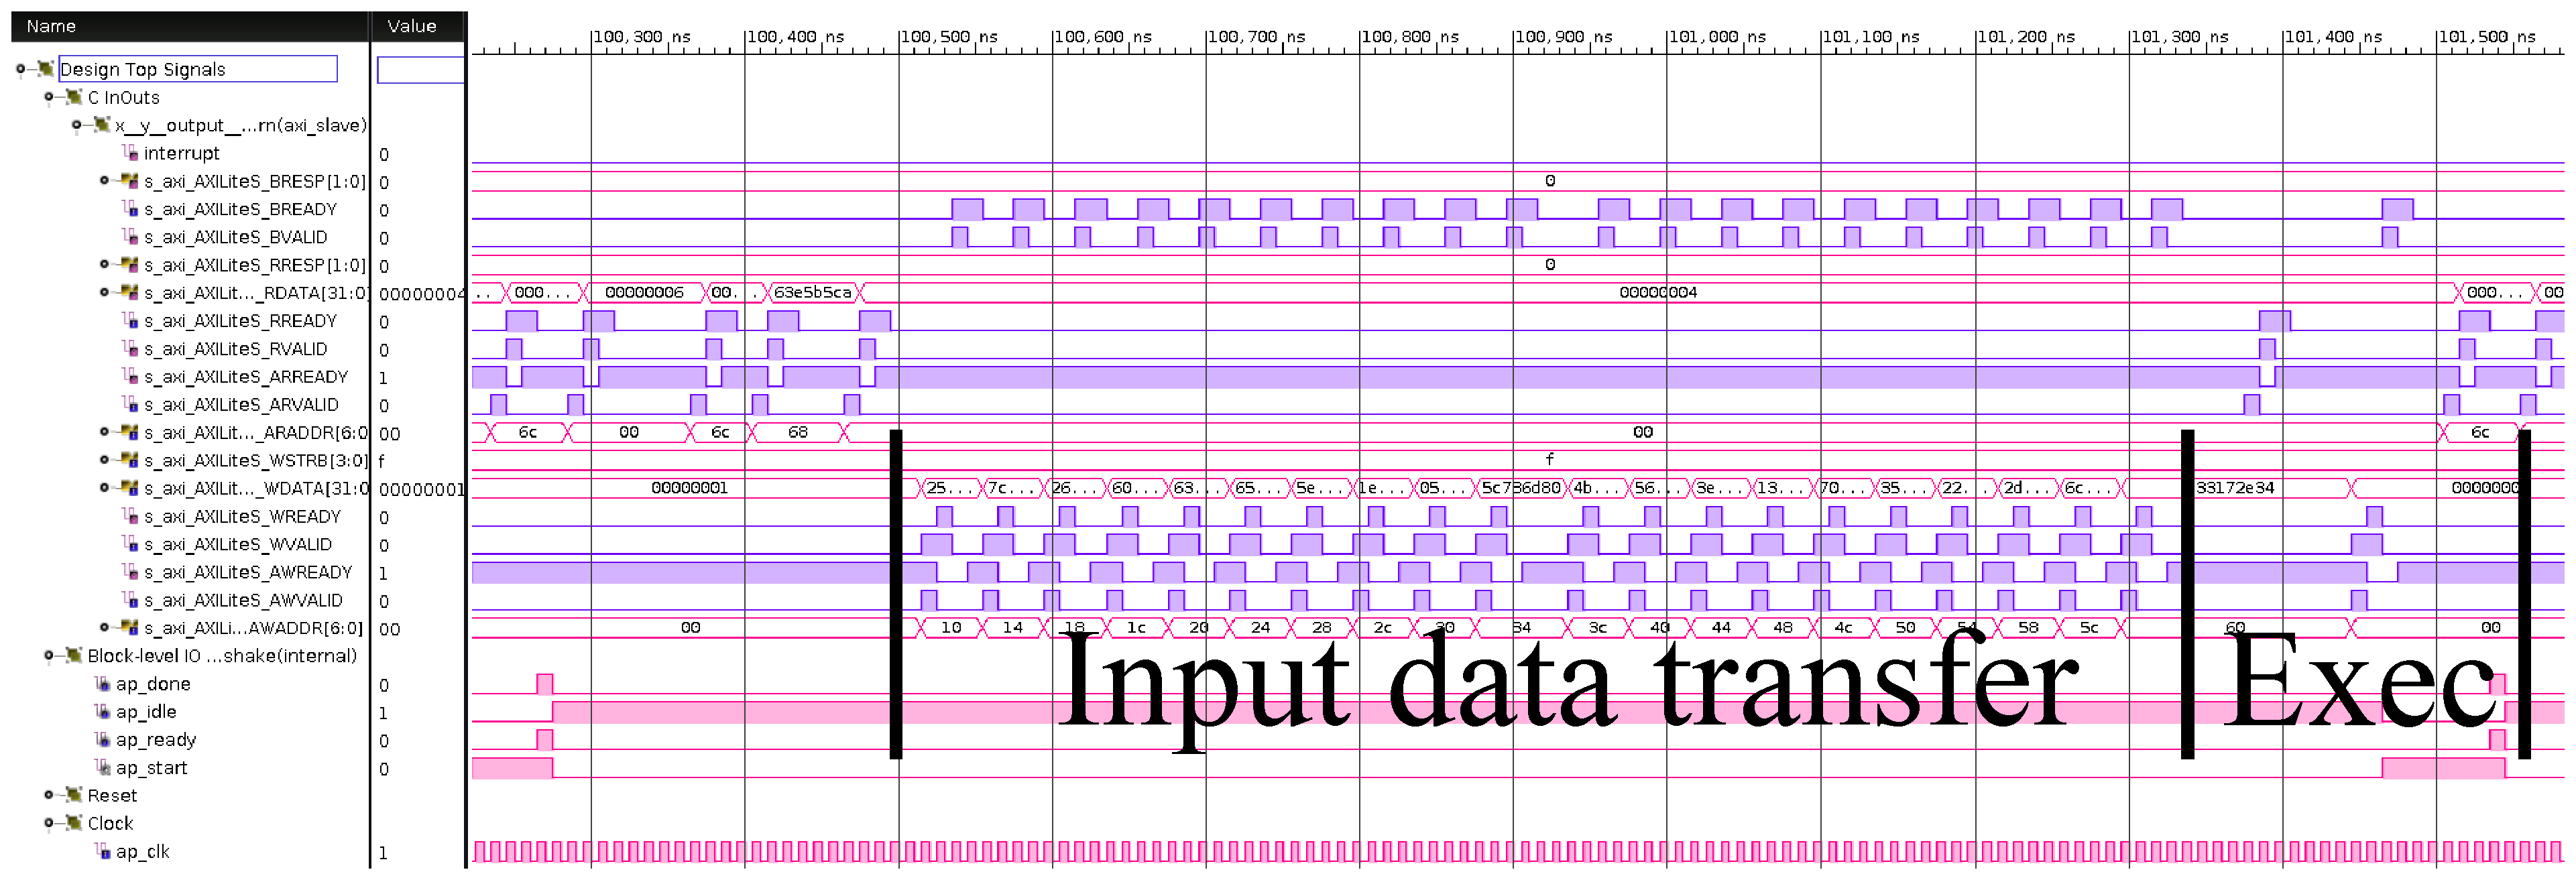
\includegraphics[width=\textwidth]{sim}
	\caption{Simulation waveform. Exec: actual execution time}
	\label{fig:sim}
\end{figure*}

The co-simulation value comes from C/RTL co-simulation process. \fref{fig:sim} shows 1 complete computation from the simulation waveform. They are about 130 cycles larger than the latency value. This is due to the inclusion of data transfers in the simulation.

\begin{figure}[!ht]
	\centering
	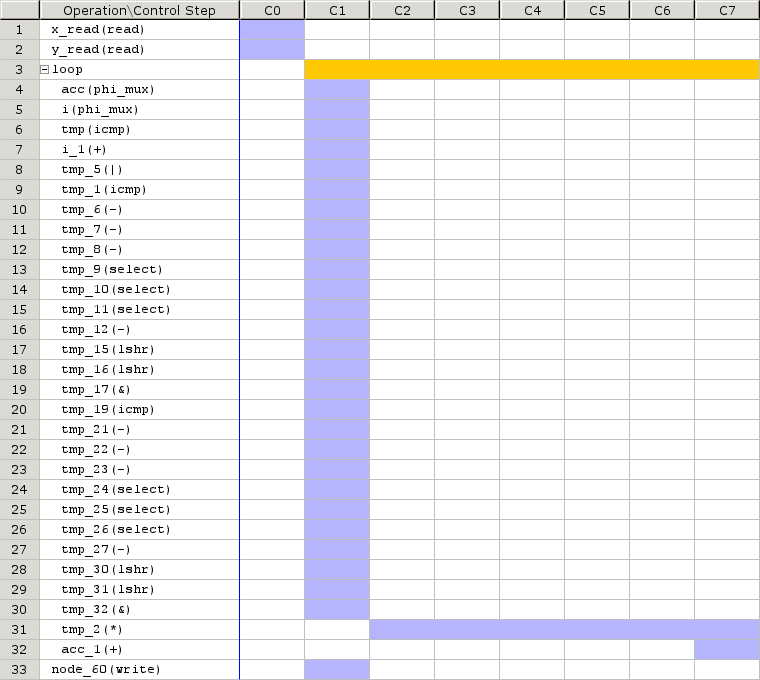
\includegraphics[width=\columnwidth]{none}
	\caption{Performance analysis of unoptimised and pipelined loop}
	\label{fig:none}
\end{figure}

\fref{fig:none} shows the control steps from the performance analysis of unoptimised and pipelined loop. They have the same structure of control steps. The difference is, unoptimised loop executes the looped steps 10 times sequentially, while pipelined loop executes the looped steps in a pipelined parallel approach. Therefore, the unoptimised loop has approximately $1 + 7 \times 10 = 71$ cycles latency, while the pipelined loop has approximately $1 + 7 + (10 - 1) = 17$ cycles latency.

\begin{figure}[!ht]
	\centering
	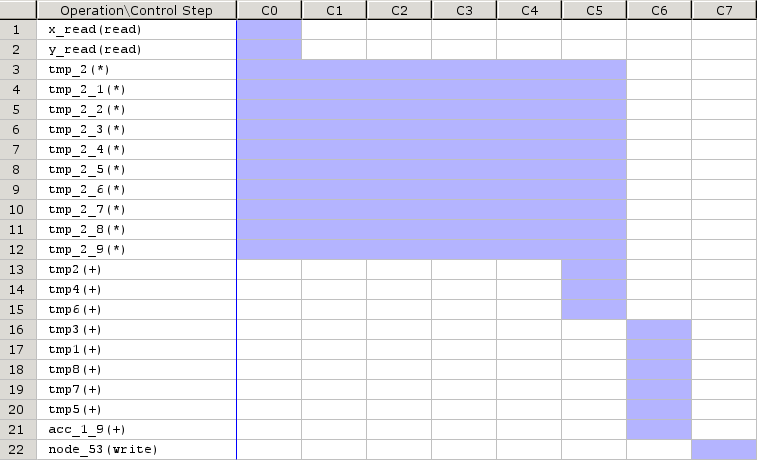
\includegraphics[width=\columnwidth]{unroll}
	\caption{Performance analysis of unrolled loop}
	\label{fig:unroll}
\end{figure}

\fref{fig:unroll} shows the control steps of the unrolled loop. All 10 iterations of the \texttt{for} loop executed in parallel by 10 multipliers realised by combinational logics, followed by combinational additions and register write back. The latency depends entirely on the propagation delay of combinational logics, which is approximately 7 cycles.

The multipliers are generated by DSP48E blocks, so the number of \texttt{UNROLL} directive uses more DSP48E blocks due to its parallel multiplication. However, the filp flops are used as registers, and look up tables (LUT) are used for combinational logics. The number of FF and LUT of \texttt{UNROLL} is much smaller than the other two directives because it does the calculation in parallel, and it does not need the logic and storage for intermediate states and buffers. 

Array related directives may also be added to the two constant sized input ports. However, the widths of the array elements matches the width of individual registers, the directives would be ineffective. 

\begin{figure*}[!t]
	\centering
	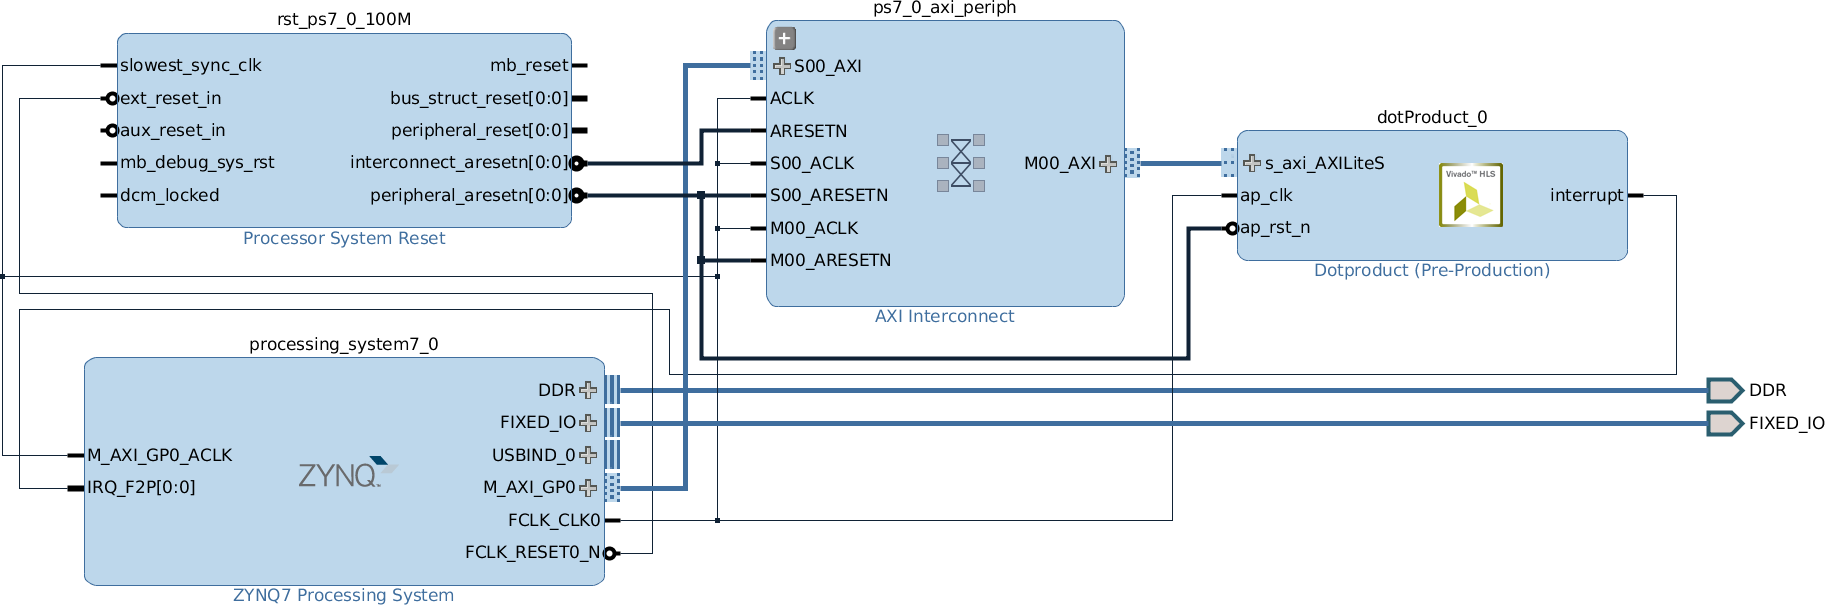
\includegraphics[width=\textwidth]{block}
	\caption{Block diagram of the system}
	\label{fig:block}
\end{figure*}

\subsection{Limitations}

This design uses a large amount of FPGA fabric resources. By optimising the range of values, i.e. optimal bit width for data types, according to the actual computation requirements which is currently unclear, the resource usage may be dramatically reduced. \tref{tbl:reswidth} shows the variations in hardware resource utilisation due to different data widths.

\begin{table}[!ht]
	% increase table row spacing, adjust to taste
	\renewcommand{\arraystretch}{1.3}
	\caption{Resource utilisation of different data width}
	\label{tbl:reswidth}
	\centering
	% Some packages, such as MDW tools, offer better commands for making tables
	% than the plain LaTeX2e tabular which is used here.
	\begin{tabular}{ccccc}
		\hline
		Data width	& BRAM\_18K	& DSP48E	& FF	& LUT	\\
		\hline
		8	& 0	& 10	& 377	& 393	\\
		16	& 0	& 10	& 697	& 745	\\
		32	& 0	& 40	& 990	& 1580	\\
		64	& 0	& 160	& 2250	& 3130	\\
		\hline
	\end{tabular}
\end{table}

\section{Software implementation}

\subsection{Hardware interfacing}

The hardware module was compiled to an IP block afterwards, and integrated to a Vivado design. \fref{fig:block} shows the block diagram of the system. The AXI4-lite interface of the module was connected to the processor through an interconnect block. The interrupt signal was connected to a fabric interrupt input \texttt{IRQ\_F2P} of the processor, signaling the completion of computation.

\subsection{Benchmarking}

A software routine was developed to evaluate the performances of hardware and software implementations. It initialises the hardware, then records the execution time of both implementations separately. The results from both implementations were also varified to ensure the currect operation of the hardware module. The timing was accomplished by using the global timer register in the ARM core. The timer is clocked at half the processor frequency.

The execution time of the hardware implementation, including data transfers, was $ticks = 1774$ and $ticks = 2327$ without and with interrupt, respectively. According to the block diagram, the processor was clocked at $f_{CPU} = 667 MHz$, while the fabric clocks at $f_{FCLK} = 100 MHz$. According to \eref{eq:clk}, the entire execution time were $532$ and $698$ fabric clock cycles.

\begin{equation}
\textrm{fabric clock cycles} = ticks * \frac{f_{FCLK}}{f_{CPU} / 2}
\label{eq:clk}
\end{equation}

However, the C/RTL co-simulation shows the complete execution cycle should be around $138$ fabric clock cycles. It is significantly different from the actual values. Therefore, the benchmarking program was modified to record more detailed time interval between function calls, as listed in \lref{lst:bm}.

\begin{lstlisting}[caption={Code segment of benchmarking program},captionpos=b,label=lst:bm]
#define USE_INTERRUPT	0

#if USE_INTERRUPT
	XDotproduct_InterruptEnable(&dotp, 1);
	XDotproduct_InterruptGlobalEnable(&dotp);
	print("Using interrupt!\n\r");
#endif

	// Reset timing
	XTime_SetTime(0);
	// Set x input data
	XDotproduct_Set_x(&dotp, x);
	XTime_GetTime(&ticks[0]);
	// Set y input data
	XDotproduct_Set_y(&dotp, y);
	XTime_GetTime(&ticks[1]);
	// Start execution
	XDotproduct_Start(&dotp);
	XTime_GetTime(&ticks[2]);
	// Waiting for result available
#if USE_INTERRUPT
	while (!ResultAvailHlsMacc);
#else
	while (!XDotproduct_IsReady(&dotp));
#endif
	XTime_GetTime(&ticks[3]);
	// Receive result
	res_hw = XDotproduct_Get_output_r(&dotp);
	XTime_GetTime(&ticks_hw);

	print("Result received.\n\r");
\end{lstlisting}

\tref{tbl:bm} shows the benchmark results translated to fabric clock cycles.

\begin{table}[!ht]
	% increase table row spacing, adjust to taste
	\renewcommand{\arraystretch}{1.3}
	\caption{Benchmarking results (fabric clock cycles)}
	\label{tbl:bm}
	\centering
	% Some packages, such as MDW tools, offer better commands for making tables
	% than the plain LaTeX2e tabular which is used here.
	\begin{tabular}{lcc}
		\hline
		& Active polling	& Using interrupt	\\
		\hline
		Transfer input x	& 211.7	& 223.2	\\
		Transfer input y	& 209.4	& 210.9	\\
		Starting execution	& 45.6	& 225.3	\\
		Result available	& 25.2	& 7.8	\\
		Transfer result		& 30.3	& 30.9	\\
		\hline
	\end{tabular}
\end{table}

The results show that the data transfer between the processor and the accelerator module was very inefficient, taking around $220$ cycles to transfer only $10$ values. The actual execution time without interrupt is still different from the $7$ cycles latency value estimated. This is because the program was polling the status of the module at fabric clock domain, thus still suffers the inefficiency of data transfer. However, the accelerator module interrupts the processor asynchronously through a signal line. This process does not involve data transfer. Therefore, the result available time is similar to the estimated latency.

The software implementation takes $51$ clock ticks to complete. This is around $15.3$ fabric clock cycles. The actual execution time of the hardware module is only about $7.8$ cycles, faster than the software implementation. However, the data transfer performance might be a limiting factor for using hardware accelerators.

\section{Conclusion}

By evaluating the performance data of software and hardware implementation of the same algorithm, the advantages, use case and limiting factors of using hardware accelerators were investigated. Although the computation speed of dedicated hardware accelerator can be faster than software implementation, the data transfer performance may limit the actual efficiency.

The data transfer inefficiency may be improved by using another type of interface, e.g. the AXI4-Stream interface. It transfers data in a sequential streaming manner, would be better than 10 discrete register data transfers.

% references section
%\bibliographystyle{IEEEtran}
%\bibliography{Reference}

% that's all folks
\end{document}
